\documentclass{article}

\usepackage[margin=1in]{geometry}
\usepackage{amsmath,amssymb}
\usepackage{graphicx}
\usepackage{algorithm, algpseudocode}
\usepackage{graphicx}
\usepackage{caption}
\usepackage{subcaption}

% commands used in algorithms
\algnewcommand{\Input}[1]{%
  \State \textbf{Inputs:}
  \Statex \hspace*{\algorithmicindent}\parbox[t]{.8\linewidth}{\raggedright #1}
}
\algnewcommand{\Initialize}[1]{%
  \State \textbf{Initialize:}
  \Statex \hspace*{\algorithmicindent}\parbox[t]{.8\linewidth}{\raggedright #1}
}

\title{SGVB ConvNets}

\author{Joost van Amersfoort \\ \\ Learning Systems Project \and Otto Fabius \\ \\ Supervised by Durk Kingma}

\begin{document}

\maketitle
\hspace{25mm} Learning Systems Project\hspace{20mm} Supervised by Durk Kingma
\tableofcontents
\newpage

\section{Introduction}
Convolutional Neural Networks (CNN's) are Neural Networks with convolutional layers, i.e. layers where the connections are such that the output of the layer corresponds to the convolution of the input with a set of learned weights. As in fully-connected Neural Networks, a point-wise non-linearity is applied after the convolution by means of an activation function. The upper limit of the performance of a CNN's is only slightly worse than that of fully-connected networks, but the weight-sharing nature of the connectivity results in much less parameters. \\
Recently, there has been much success in applying CNN's to image processing tasks such as classification (Krizhevsky), detection, and localization (OverFeat). This succes can mostly be attributed to an increase in the amount of available annotated data, the steady increase in computing power, and efficient implementations on GPU's. These CNN's are trained on a supervised error criterion, such as Binary Cross-Entropy on class labels for classification tasks (e.g. ...., OverFeat) or logistic regression on x-y coordinates for localization tasks (OverFeat).\\
However, so far there has only been success in the supervised training of such networks. Unsupervised training of CNN's, although desirable for a multitude of reasons (........ergens moet staan welke allemaal! Discussie of intro?...........), has not yet been done successfully. The most popular approach for unsupervised training of deep, fully-connected Neural Networks is layer-wise, by means of RBM's (Hinton refs ofzo). This technique is restricted to fully-connected layers and can therefore not be applied to CNN's. Recently, however, Kingma and Welling developed an effective, efficient method to perform approximate inference with Variational Bayes by means of stochastic gradient ascent on the variational lower bound. Stochastic Gradient Variational Bayes (SGVB) has been successfully applied to unsupervised training of fully-connected neural networks (Kingma and Welling), and first empirical results show that, for the tasks investigated, this outperforms RBM's (internal communication). \\
In the current work, we will make the first steps in investigating whether and how SGVB can be used with a CNN as encoding network. Since this method requires both an encoding network and a (generative (moet dit hier of bij volledige network??) decoding network (ref durk?), we will refer to the full model as a Deconvolutional Neural Network (DNN). (....hier past nog wel een link naar zeilers deconvnet?)


\subsection{This Project}
Firstly, we will briefly describe the framework we use to implement the DNN(s), as this is relevant for the choice network architectures. Next, we will describe the experiments we ran to answer our research questions. As DNN's have never been trained before (nb zeiler), our first question is how to perform deconvolution, i.e. what network architecture to use for the decoder. Next, we will investigate what network architectures can be trained efficiently, and how effective they are. Where appropriate, we will compare the results to similar, fully connected models. Finally, we discuss the results and make recommendations for further research on this topic.
\newpage





%\section{Deconvolutional Neural Networks with SGVB}
%In their paper, Kingma and Welling (ref) used a reparametrization technique to obtain unbiased, stochastic gradient to perform Variational Bayes. Here, the data $\mathbf{X}$ is assumed to be generated by some underlying random process which involves unobserved, or latent, continuous variables $\mathbf{z}$. The conditional probability $p(\mathbf{X}|\mathbf{z})$ and $q(\mathbf{z}|\mathbf{X})$ (the approximation of $p(\mathbf{z}|\mathbf{X})$) are modeled by fully-connected neural networks. These networks can be referred to as \textit{encoder} and \textit{decoder}, respectively, which can be nderstood by viewing the latent representation $\mathbf{z}$ of the data $\mathbf{X}$ as a code as in coding theory (ref). \\
These networks are trained using stochastic gradient descent on the lower bound:

\begin{align}
\mathcal{L}(\mathbf{\theta}, \mathbf{\phi}; \mathbf{X}) = \log p_\theta(\mathbf{X}) - D_{KL}(q_\phi(\mathbf{z}|\mathbf{X}) || p_\theta(\mathbf{z}|\mathbf{X}))
\end{align}

In order to obtain estimates of the derivative of $\mathcal{L}(\mathbf{\theta}, \mathbf{\phi}; \mathbf{X})$, $\mathbf{z}$ is sampled from the deterministic function $g_{\theta}(\epsilon,\mathbf{x})$, which depends on sampled noise $\epsilon \sim N(0,1)$. This is an effective, efficient method for unsupervised training of neural networks. Furthermore, the resulting model is generative, which comes with many advantages. \\
The approach we take in this project is very similar. The main difference is that in stead of using one or more fully connected layers to model $q(\mathbf{z}|\mathbf{X})$, convolutional layers are used. This means that for the decoder to model $p(\mathbf{X}|\mathbf{z})$ effectively, it needs to be capable of some form of deconvolution to reconstruct the data $\mathbf{X}$ from $\mathbf{z}$. 


\section{Implementation}\label{implementation}
In this section our implementation is detailed. We begin by explaining what framework we used and what additions were necessary to implement SGVB. Furthermore, we explain how the framework makes it possible to train networks on the GPU. 

\subsection{Torch7}

Torch7 \cite{collobert2011torch7} is a Machine Learning library written in Lua and C specifically for Neural Networks. Most code is written in C, which interfaces great with Lua and the efficient LuaJIT. In Torch7 it is simple to define a Neural Network, first one defines the type of model (usually Sequential) and then it is possible to stack modules. Examples of a few modules are Sigmoid, Rectified Linear Unit, Convolution and Max Pooling. Finally it is necessary to define a criterion, or objective function, such as the MSEcriterionn. This way of defining a module makes it easy to iterate through many different versions. For example changing the activation function is just one line of code. Also relative to Theano (the other major library used for this purpose) debugging is more straight-forward as the code does not go into a compilation phase.

In order to implement SGVB it was necessary to create several new modules. The first of these modules is the Reparemtrize step, which, in the case of a Gaussian function for g, takes two inputs: the mean and the standard deviation. The output are then samples of this Gaussian made with the noise parameter $\epsilon$. The second module that was not readily available in Torch7 was the Binary Cross Entropy, necessary to compute the reconstruction error after a forward pass through the network. We submitted this module to the authors of Torch7 and it is now part of the standard library.


\subsection{CUDA}

Another benefit of Torch7 is its support for running on the GPU, because most of the commonly used modules are implemented in CUDA, the language used by nVidia graphic cards. In order to make efficient use of CUDA we had to rewrite our modules to only use Torch7 functions that have a CUDA implementation. Without any other changes than rewriting the modules we were able to get a 2 to 3x speed up. After rethinking the structure of our networks and making some vital changes, such as increasing the mini-batch size to 128 and using a convolution module specifically written for the GPU, we managed to get 10 to 20x speed ups.

Unfortunately, as all calculations done by Torch7 on the GPU are in single precision, the network became more unstable. We had to decrease the learning rate and try to use SGD instead of AdaGrad as a means to update the parameters.


\newpage

\section{Model Specifics}\label{model_specs}
\subsection{General Network Architecture}
General convnet stuff, number of feature maps, map sizes etc

\subsection{Deconvolution}
How to do this

\subsection{Hidden Space}
not sure if this needs a separate subsection

\subsection{Miscellaneous Hyperparameters}
m.n. learningrate, adagrad

\newpage

\section{Results}\label{results}
\subsection{MNIST}

\subsubsection{1 layer}


\begin{figure}
	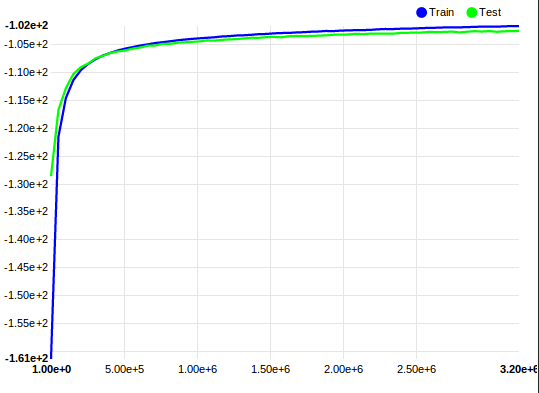
\includegraphics[scale=0.8,trim=0cm 0cm 0.1cm 0cm, clip=true]{images/MNIST_28_conv_nocuda.png}
	\caption{Lower bound for a one-layer DNN without subsampling trained on MNIST. A Spatial Convolution was also used in the Deconvolutional layer.}
	\label{label1}
\end{figure}

\subsubsection{2 layers}

\subsubsection{Overview}

Table \ref{overview} shows an overview of the results for MNIST experiments. 
\begin{table}
\caption{Overvieuw of results on MNIST. The Deconvolution Method row specifies which method, as described in Section 4.2, is used in the decoder.}
\renewcommand{\arraystretch}{1.5}
\label{overview}
\begin{tabular}{| l | l | l | l | l | l | l | l | l |}

	\hline
  Number of layers 					& 1 	 	& 1 		& 1 		& 2 		& 2 			& 2 		& .. \\ \hline
  Feature map size 					& 7 		& 14 	& 28 	& 14-7	& 14-14		& 14-14 	& .. \\ \hline
  Deconvolution Method 				& MLP 	& MLP	& Conv 	& MLP	& MLP\& Conv	& MLP	& ..	 \\ \hline
  Total number of parameters 		& .. 	& .. 	& ..		& ..		& ..			& .. 	& .. \\ \hline
  Train lower bound 					& 108.9 	& 102.8 	& 101.3 	& 126.7*	& ..			& ..		& .. \\ \hline
  Test lower bound 					& 109.5	& 103.7 	& 102.3 	& 126.5*	& ..			& ..		& .. \\ \hline
  %1 & 28 	& SpatialConvolution 	& .. & .. 	& -.. \\ \hline
  %1 & 28 	& MLP					& .. & .. 	& -.. \\ \hline
  %1 & 14 	& MLP 					& .. & .. 	& -.. \\ \hline
  %1 & 7  	& MLP 					& .. & .. 	& -.. \\ \hline
  %2 & 14 14 	& SpatialConvolution 	& .. & .. & -.. \\ \hline
  %1 & 28 14	& SpatialConvolution 	& .. & .. & - N/A \\ \hline
  %1 & 14 7 	& SpatialConvolution 	& .. & .. & - N/A \\ \hline
\end{tabular}
\end{table}


\subsection{CIFAR-10}






%%%%%%%%%%%%%%%%%%%%%%%%%%%%%%%%%%%%%%%%%%
\begin{figure}
	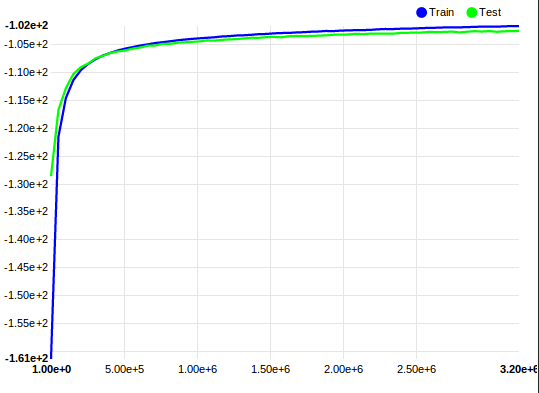
\includegraphics[scale=0.1]{images/MNIST_28_conv_nocuda.png}
	\caption{blablabla}
	\label{label1}
\end{figure}

\begin{figure}
	\centering
	\begin{subfigure}[b]{0.3\textwidth}		
		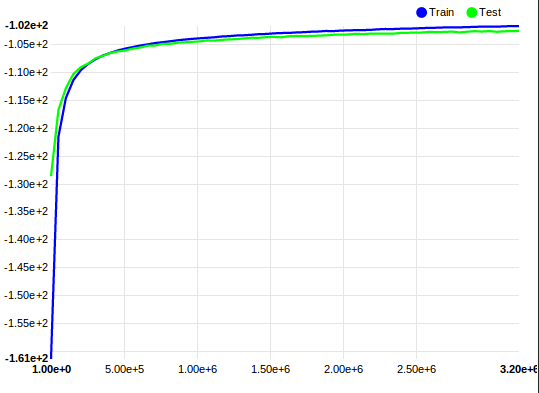
\includegraphics[scale=0.1]{images/MNIST_28_conv_nocuda.png}
		\caption{blablabla}
	\end{subfigure}

	\begin{subfigure}[b]{0.3\textwidth}		
		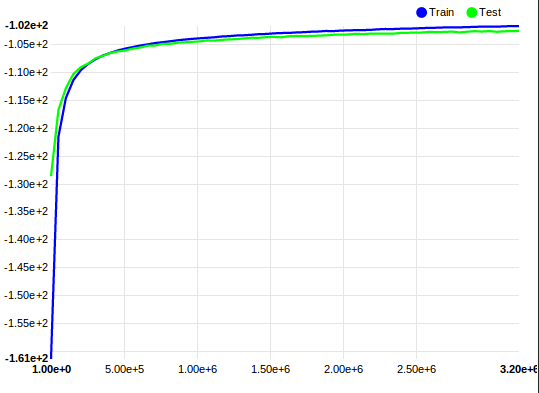
\includegraphics[scale=0.1]{images/MNIST_28_conv_nocuda.png}
		\caption{blablabla}
	\end{subfigure}
	\label{label2}
\end{figure}
\newpage




\section{Discussion and Future Work}\label{discussion}
short recap

\subsection{Comparison with fully connected MLP}
Even though multiple convolutional layers are often used in CNN's, a one-layer DNN is potentially interesting as an encoder because the number of weights is lower than in traditional auto-encoders due to weight-sharing. 
\subsection{Future Work}

%bugs: 
%-spatialconvolutionCUDA doesn't work for 1-layer-7, where SpatialZeroPadding does work


\newpage

\section{Conclusion}\label{conclusion}
\subsection{subsection title}


Machine Learning is hard


\pagebreak 
\nocite{*}
\bibliographystyle{amsplain}
\bibliography{ref}

\end{document}
